\documentclass{article}
\PassOptionsToPackage{numbers,sort&compress}{natbib}
\usepackage[preprint]{neurips_2026}
\usepackage[T1]{fontenc}
\usepackage[utf8]{inputenc}
\renewcommand{\ttdefault}{lmtt}
\usepackage{amsmath,amssymb,amsthm,booktabs,array,graphicx,microtype}
\usepackage[dvipsnames]{xcolor}
\usepackage[hyphens]{url}
\usepackage[colorlinks=true,linkcolor=MidnightBlue,citecolor=MidnightBlue,urlcolor=MidnightBlue]{hyperref}
\usepackage{enumitem}
\setlist[itemize]{itemsep=1pt,topsep=3pt,leftmargin=1.5em}
\setlist[enumerate]{itemsep=1pt,topsep=3pt,leftmargin=1.5em}
\newtheorem{proposition}{Proposition}
\newtheorem{definition}{Definition}
\newcommand{\code}[1]{\texttt{#1}}
\newcommand{\ind}{\mathbf{1}}
\newcommand{\botval}{\bot}
\newcommand{\evalcommit}{\code{a18a070}}
\newcolumntype{L}[1]{>{\raggedright\arraybackslash}p{#1}}
\hypersetup{pdftitle={Evidence Roles and Answer Contracts in Data Analysis Agents},pdfauthor={Yiting Feng},pdfsubject={Research draft: conditional interface properties and a small same-build validation}}
\title{Evidence Roles and Answer Contracts\\in Data Analysis Agents}
\author{Yiting Feng}
\begin{document}
\maketitle

\begin{abstract}
A data-analysis agent can compute the right value in the wrong artifact, or explain a correct table incorrectly. We study an interface that separates one primary answer from supporting evidence and checks a caller-frozen contract before accepting an answer-bearing finish. We formalize its acceptance predicate and show, under explicit assumptions, that acceptance certifies recorded-result structure but cannot certify semantics. A finite-budget model separates recoverable rejection from guaranteed completion. In three prospective question families on an adapted BIRD Mini-Dev database, the combined role/contract interface passes the strict endpoint on 3/3 families, versus 2/3 for same-build legacy mode. Both modes supply all three correct substantive answers. The difference is one repaired shape violation, at 14 versus 11 requests and CNY 0.102346 versus 0.079332. Separately, an exposed regression returns a correct 19-row ranking but miscounts its singleton categories in prose. Across all 13 declared trials, 29 distinct captured query results replay correctly. The study supports one observed structural-compliance benefit while identifying narrative grounding as an independent failure mode. It establishes neither statistical superiority nor a general accuracy guarantee.
\end{abstract}

\section{Introduction}
Data-analysis agents produce selected tables, auxiliary evidence, assumptions, and narrative conclusions. Each component imposes a different obligation: the artifact must have the requested form, its values must answer the question, and its explanation must follow from the evidence. Successful query execution alone establishes none of these obligations.

Consider a consumer expecting one integer column, \code{publisher\_id}. An agent may compute the right identifier but return an extra publisher-name column. A human can recover the answer, yet the artifact violates the consumer's interface. Conversely, an incorrect identifier can have exactly the required shape. A third failure occurs when a correct ranking is summarized inaccurately. Downstream software and human readers may rely on different components.

Workflow Data Investigator exposes an optional answer contract and explicit evidence roles~\citep{wdidocs}. The caller fixes column names, types, nullability, and row-count bounds before a run. The agent designates one query as its answer and other records as support. Rejection returns actionable feedback while the original budget permits another step. The contract contains no expected values or reference SQL, so it enforces an interface obligation rather than numerical truth.

This paper contributes (1) a formal interface model with elementary conditional propositions delimiting acceptance and repair, (2) a three-family, same-build comparison of the combined role/contract/instruction change, and (3) independently checked structural, numerical, and narrative outcomes with two failure analyses. It is an engineering characterization and small case study, not a new learning algorithm or formal verification of the software.

\paragraph{Research status.} Draft dated 12 October 2026, in the official NeurIPS preprint style; not a submitted or accepted conference paper. Evaluation is bound to commit \evalcommit. Appendix~\ref{app:provenance} distinguishes current documentation.

\section{Evidence roles and the answer contract}
\label{sec:method}
\subsection{A primary answer and inspectable support}
The explicit finish interface distinguishes an answer-bearing report from a request for clarification. An \code{answered} or \code{conditional} finish requires one primary query result. Support is a separate list of current-run evidence identifiers; it can include successful query results, context reads, schema inspection, analysis, or plots. A \code{needs\_clarification} finish can omit the primary when its support and retained blocker satisfy the interface rules. Our structural acceptance statements below concern answer-bearing finishes.

Every referenced query, whether primary or supporting, must be successful and untruncated, with a recorded row count equal to the stored number of rows. All supporting records must be successful and belong to an allowed evidence kind. Supporting identifiers must be distinct and cannot repeat the primary identifier. Only the primary must satisfy the answer contract. Checking a support identifier establishes that the record exists and is structurally usable; it does not establish its relevance to a claim.

The caller's contract is validated and reconstructed before model execution, isolating the run from later mutation of the original caller object. This is an ownership boundary, not immutability against a trusted host that deliberately modifies runtime state. The model's finish payload and input documents cannot redefine the contract through the exposed tool interface.

\begin{figure}[t]
\centering
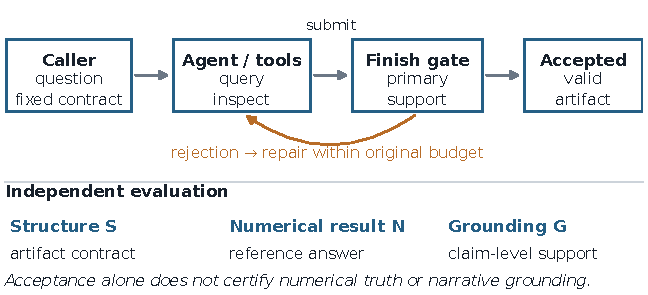
\includegraphics[width=\linewidth]{figures/interface-verification.pdf}
\caption{The answer-bearing finish path and its verification boundaries. The upper row is a conceptual interface schematic. Rejection can feed another agent step only while the original budget and runtime phase permit it. The lower row shows separate post-run checks; runtime acceptance alone certifies neither numerical truth nor narrative grounding.}
\label{fig:interface}
\end{figure}

\subsection{Formalizing structural eligibility}
Let $E$ map current-run evidence identifiers to recorded objects. A query object $e$ has ordered column names $\operatorname{cols}(e)$, rows $R_e$, a success flag, a truncation flag, and a recorded row count $n_e$. Define query completeness as
\begin{equation}
\operatorname{Complete}(e) := \operatorname{query}(e)\land\operatorname{ok}(e)
\land\neg\operatorname{truncated}(e)\land (n_e=|R_e|).
\label{eq:complete}
\end{equation}
The definition presumes well-formed row storage and an integer recorded count; it is a predicate on the captured object, not on an unobserved database response.

A contract is $C=(\mathbf c,\boldsymbol\tau,\boldsymbol\nu,\ell,u)$, where $\mathbf c=(c_1,\ldots,c_d)$ is an ordered list of distinct column names, $\tau_j$ is a supported value type, $\nu_j\in\{0,1\}$ permits nulls, and integer bounds satisfy $0\le\ell\le u\le200$. The implementation permits $1\le d\le64$. Let $T_{\tau}(v)$ denote the implementation's value-type predicate and write $r_j=r[c_j]$. Define
\begin{align}
\operatorname{Shape}_C(e) := {}& [\operatorname{cols}(e)=\mathbf c]\land[\ell\le |R_e|\le u] \notag\\
&\land\!\bigwedge_{r\in R_e}\!\left[\operatorname{keys}(r)=\{c_1,\ldots,c_d\}\right] \notag\\
&\land\!\bigwedge_{r\in R_e}\bigwedge_{j=1}^{d}
\left[(r_j=\mathrm{null}\land\nu_j=1)\lor(r_j\ne\mathrm{null}\land T_{\tau_j}(r_j))\right],
\label{eq:shape}\\
V_C(e) := {}&\operatorname{Complete}(e)\land\operatorname{Shape}_C(e).
\label{eq:valid}
\end{align}
The ordered column list and each row's key set serve different checks. Neither specifies which rows should have been selected, how ties should be ranked, or what the values should be.

Write an answer-bearing submission as $z=(p,W,h)$, with primary identifier $p$, support list $W$, and remaining report fields $h$. Let $R_E(p,W)$ require that all identifiers resolve within $E$, all supports are successful records of allowed kinds, the support list is duplicate-free, $p\notin W$, and every query support passes Equation~\eqref{eq:complete}. Let $K_E(z)$ collect the remaining payload, status, and retained-blocker checks. A faithful abstraction of acceptance is
\begin{equation}
A_C(E,z)=\ind\{p\in\operatorname{dom}(E),\ V_C(E[p]),\ R_E(p,W),\ K_E(z)\}.
\label{eq:gate}
\end{equation}
Equation~\eqref{eq:gate} intentionally leaves status-specific policy in $K_E$ rather than treating a valid table as sufficient for acceptance.

\subsection{Conditional properties and their limits}
\label{sec:theory}
The following statements are elementary consequences of the model. They specify interface guarantees under stated assumptions; they are not novel generalization results or machine-checked claims about every execution.

\begin{proposition}[Recorded structural soundness]
\label{prop:sound}
Assume (i) identifier lookup returns the intended current-run records, (ii) the contract remains fixed across validation and acceptance, and (iii) the gate implements Equation~\eqref{eq:gate} soundly. If an answer-bearing finish is accepted, then its primary satisfies $V_C$, its support identifiers resolve without role conflicts, and all referenced query records are complete.
\end{proposition}
\begin{proof}
Acceptance makes each conjunct of Equation~\eqref{eq:gate} true. Expanding $V_C$ gives completeness and every shape constraint; expanding $R_E$ gives reference, uniqueness, role-separation, and query-support conditions. No semantic conclusion appears in these conjuncts.
\end{proof}

\begin{proposition}[Shape checks cannot certify semantics]
\label{prop:semantic}
Let $g(e)$ be the vector of properties inspected by a shape-only validator. If two records satisfy $g(e)=g(e')$ but their answer-correctness labels differ, every deterministic validator that depends only on $g$ assigns them the same decision. In particular, accepting the correct record also accepts the incorrect one.
\end{proposition}
\begin{proof}
A shape-only decision has the form $f(g(e))$. Equal inputs to $f$ give equal outputs, regardless of the correctness labels. For a concrete witness, one-row, one-column successful integer results containing 20 and 21 have the same relevant shape, although only one may answer the question. Similarly, changing report prose while retaining a valid table can change grounding without changing $V_C$.
\end{proof}

A valid contract can still reduce a useful class of failures: the extra-column artifact in task 745 is excluded even though it contains the right identifier. Proposition~\ref{prop:semantic} explains why an excluded structural failure and an undetected semantic failure can coexist. Contract expressiveness, numerical verification, and claim checking address different sets of errors.

\subsection{Budgeted rejection and repair}
Represent the control state by $s_t=(E_t,C,b_t,m_t)$, where $b_t$ records remaining resources and $m_t\in\{\mathrm{normal},\mathrm{finish\mbox{-}only},\mathrm{terminal}\}$. An ordinary rejected finish records an error observation and can return control to the agent. A rejected finish-only submission terminates under the existing runtime rules. In either case the attempt remains part of the same trial; the contract and original caps do not reset.

\begin{proposition}[Bounded continuation without guaranteed repair]
\label{prop:bounded}
Assume finite original model-turn and tool-action caps, no reset of those caps after rejection, and that every additional model request consumes one remaining model turn. If $k$ model turns remain after a rejection, at most $k$ further model requests can occur. A finish-only rejection permits no further repair request under the modeled transition rule. Neither condition guarantees an accepted finish.
\end{proposition}
\begin{proof}
The remaining-turn count is a nonnegative integer that decreases by one with each additional request, so it can decrease at most $k$ times. Other limits may stop execution earlier. The finish-only rejection transition is terminal by definition. Repeated structurally invalid submissions can exhaust the budget without acceptance. Separately, a wrong but structurally valid answer can be accepted; the bound gives no correctness guarantee.
\end{proof}

For model-request count $r$ and nonnegative per-request costs $c_t$, an in-trial repair contributes to the same totals,
\begin{equation}
\operatorname{Cost}=\sum_{t=1}^{r}c_t,\qquad r\le B_{\mathrm{turn}}.
\label{eq:cost}
\end{equation}
Thus the relevant empirical question includes both failure exclusion and its observed resource cost. It cannot be resolved from structural soundness alone.

\section{Evaluation protocol}
\label{sec:protocol}
\subsection{Same-build comparison and declared panels}
Both modes use source commit \code{a18a07061ea7b9a3e1950b4527e36e266d17b487}. Legacy mode retains the earlier finish interface. Explicit mode combines evidence-role fields, a caller-frozen contract, and corresponding instructions. Modes, case order, contracts, and resource caps were declared before the evaluated phase. The design does not isolate the causal effect of each component, and the fixed order was not randomized.

The model configuration uses provider alias \code{deepseek-flash}, temperature 0, disabled thinking, automatic tool choice, and non-streaming responses. No seed or top-$p$ is specified, and the alias is not an immutable model version. The database is an adapted five-table projection from BIRD-SQL Mini-Dev with source rows preserved~\citep{birdminidev}. The database was already known during development. Here, \emph{prospective} means question families declared for this phase, not an unseen database, a contamination test, or an official BIRD benchmark score.

\begin{table}[t]
\caption{Declared evaluation panels. Only the first row supplies the matched fresh-family comparison. The other panels retain useful diagnostics and exposed failures without expanding that denominator.}
\label{tab:panels}
\centering\small
\begin{tabular}{@{}L{1.20in}L{1.38in}L{1.70in}r@{}}
\toprule
Panel & Task identifiers & Modes & Trials\\
\midrule
Prospective families & 744, 745, 800 & Legacy and explicit & 6\\
Related diagnostic & 829 (related to 744) & Legacy and explicit & 2\\
Exposed smoke & 764 & Explicit & 1\\
Exposed regressions & 723, 728, 733, 765 & Explicit & 4\\
\bottomrule
\end{tabular}
\end{table}

Table~\ref{tab:panels} accounts for all 13 declared trials. Each assigned mode and task is run once. The three prospective families are scalar-result tasks. Ranking and multirow coverage comes from exposed development material. Historical October 11 full/minimal strict results of 2/4 versus 3/4 are a separate study and are neither rescored nor pooled here.

\subsection{Selection and success criteria}
The evaluator applies a frozen primary-selection rule to the final cited evidence before comparing an eligible result with its reference. Explicit mode supplies the primary role directly; legacy mode is assessed for a uniquely eligible cited primary under the predeclared shape rule. If no unique eligible primary exists, the numerical grade is $\botval$ (unverifiable), even when prose supplies the correct answer. An earlier query or a correct sentence is not promoted post hoc to rescue the artifact grade.

Formally, let $\sigma(E,z,C)$ be that predeclared selection rule. Numerical verification is a partial outcome,
\begin{equation}
N=\begin{cases}
\ind\{\operatorname{rows}(\sigma(E,z,C))\equiv y^\star\}, & \sigma(E,z,C)\ne\botval,\\
\botval, & \sigma(E,z,C)=\botval,
\end{cases}
\label{eq:numerical}
\end{equation}
where $y^\star$ is the frozen reference and $\equiv$ uses the required typed-result and ordering semantics. Selection does not inspect $y^\star$. Consequently, replacing the reference alone cannot change the selected artifact. Conditional on a fixed contract and selector, this prevents gold-driven rescue at the evaluator stage; it does not establish correctness or absence of upstream answer leakage.

We record native finish acceptance $F$, structural eligibility $S$, reference-correct primary $N$, full-question completion $Q$, grounding $G$, number of unsupported or contradicted claims $U$, and resource/policy compliance $P$. The strict endpoint is
\begin{equation}
Y=\ind\{F=1,\ S=1,\ N=1,\ Q=1,\ G=1,\ U=0,\ P=1\}.
\label{eq:endpoint}
\end{equation}
An unverifiable primary cannot pass $Y$, but is not mislabeled as a wrong numerical result. Complete substantive answers are also examined as a separately labeled diagnostic; this does not relax Equation~\eqref{eq:endpoint}.

\subsection{Independent checks}
The mechanical review rehashed 62 evidence objects and six contracts, verified within-trial identifier resolution, retained all 17 finish attempts, and checked terminal tool outcomes against accepted-finish flags. It replayed all 29 distinct captured SQL results read-only against the hash-verified projection. All matched as typed multisets; ordering requirements were checked without imposing arbitrary order among ranking ties.

An AI-assisted review, blinded to mode and status labels, assessed full-question completion and decomposed narrative claims into 114 atoms. It was not human expert annotation, and content could reveal related cases. Six grain/key claims relied on available source context rather than a dedicated cited query. Documented source keys were distinguished from constraints not recreated during CSV import. These qualifications matter when interpreting grounding counts.

\section{Results}
\label{sec:results}
\subsection{One paired structural difference}
\begin{figure}[t]
\centering
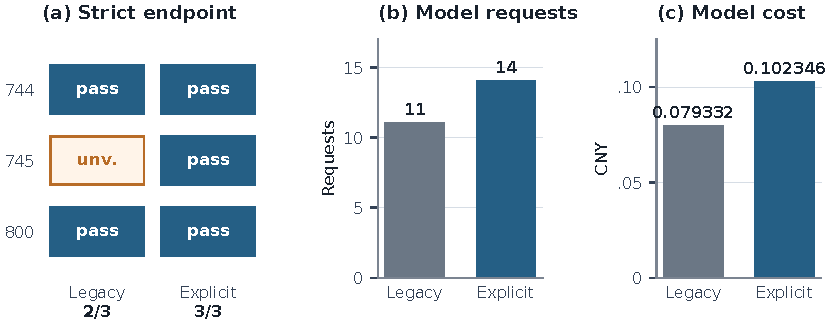
\includegraphics[width=\linewidth]{figures/prospective-results.pdf}
\caption{Three prospective families, one trial per mode and family. (a) Strict outcomes show one explicit-mode win and two ties; ``unv.'' denotes the legacy primary that is structurally unverifiable. Both modes answer all three substantive questions correctly. (b--c) Explicit mode uses more requests and higher recorded model cost. These are descriptive counts and sums, not population estimates or significance tests.}
\label{fig:prospective}
\end{figure}

Explicit mode passes the strict endpoint on 3/3 prospective families; legacy mode passes on 2/3 (Figure~\ref{fig:prospective}; Table~\ref{tab:primary}). The matched outcomes are one explicit-mode win, zero legacy-mode wins, and two ties. Both modes return complete correct substantive answers, and neither has an unsupported prospective narrative claim under the review. There is no observed arithmetic-accuracy improvement.

\begin{table}[t]
\caption{Prospective outcomes and resources. ``Unverifiable'' is distinct from an incorrect eligible answer. Costs include within-trial rejected finishes.}
\label{tab:primary}
\centering\small
\begin{tabular}{@{}L{3.32in}rr@{}}
\toprule
Measurement & Legacy & Explicit\\
\midrule
Reference-correct selected primary ($N=1$) & 2/3 & 3/3\\
Unverifiable selected primary ($N=\botval$) & 1/3 & 0/3\\
Incorrect eligible selected primary ($N=0$) & 0 & 0\\
Complete substantive answers & 3/3 & 3/3\\
Native accepted finishes ($F=1$) & 3/3 & 3/3\\
Conforming selected primaries ($S=1$) & 2/3 & 3/3\\
Reports containing unsupported claims ($U>0$) & 0/3 & 0/3\\
Strict end-to-end success ($Y=1$) & 2/3 & 3/3\\
\midrule
Model requests & 11 & 14\\
Recorded model cost (CNY) & 0.079332 & 0.102346\\
\bottomrule
\end{tabular}
\end{table}

Task 745 accounts for the difference. Its contract requires a one-row result with \code{publisher\_id} alone. Explicit mode first submits two columns, receives a column-mismatch rejection, and repairs the artifact within the original trial. Legacy mode accepts a two-column result containing the correct identifier 20 and publisher name. Its final prose and cited identifier are correct as diagnostics, but no unique eligible one-column primary exists under the frozen selection rule. Its structural and numerical grades remain unverifiable.

This case directly illustrates Proposition~\ref{prop:sound}: a contract violation is excluded at the explicit gate and corrected before acceptance. The evidence does not attribute that correction separately to role names, instructions, or validation feedback. It also does not establish that a consumer unconcerned with output shape would prefer the additional enforcement.

\subsection{A correct ranking with a contradicted summary}
\label{sec:regression}
All four exposed regressions have accepted finishes, conforming selected primaries, correct selected results, and complete substantive answers. Strict success is nevertheless 3/4. In task 728, the complete 19-row ranking is correct, while the summary states that six colours are tied at count 1. The table contains seven such colours: Yellow/Blue, White/Red, Violet, Silver, Green/Blue, Blue/White, and Amber (Figure~\ref{fig:ranking}).

\begin{figure}[t]
\centering
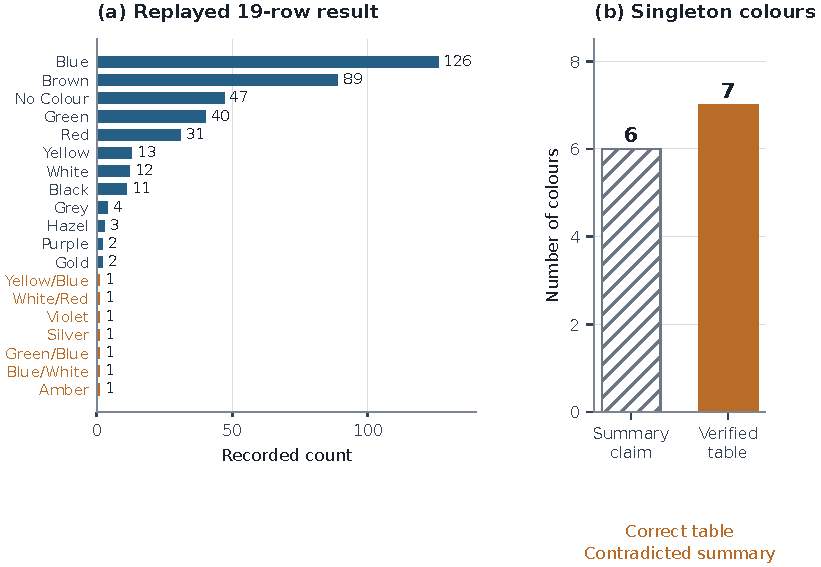
\includegraphics[width=\linewidth]{figures/ranking-grounding-failure.pdf}
\caption{Exposed regression 728 separates numerical truth from narrative grounding. (a) All 19 ranking rows replay correctly; the seven count-1 colours are highlighted. The figure preserves the recorded within-tie display order without requiring that order for grading. (b) The submitted summary claims six singleton colours. The requested ranking is complete, so $Q$ passes; the contradicted summary fails grounding and the strict endpoint.}
\label{fig:ranking}
\end{figure}

The error is not a hidden failure of the selected table. It is a contradiction in another component of the report. This supplies a concrete instance of Proposition~\ref{prop:semantic}: holding a numerically correct, structurally accepted artifact fixed does not determine the truth of its summary. A reader who relies on the summary may still receive an incorrect statement.

\subsection{Remaining panels and retained attempts}
Both modes pass the related sign diagnostic 829, and the exposed smoke task 764 passes. Descriptively across all 13 mixed-panel trials, native acceptance is 13/13, structural eligibility is 12/13, all 12 eligible selected results match the references, full-question completion is 13/13, and strict success is 11/13. Because mode assignments differ by panel, these mixed totals are not an ablation score.

All four rejected finish attempts remain in the record: three duplicate-support-ID errors and the task-745 column mismatch. They are repaired within their original trials. No paid trial reruns or API retries are recorded. In-trial repair therefore contributes to both the final outcome and the resources consumed, rather than being counted as a new independent sample.

The narrative review identifies 113 supported atoms and one contradicted atom among 114 (0.88\%). The ranking report contributes 46 atoms, including the contradiction. This atom-level denominator is highly uneven across reports. A single contradicted atom fails that report's strict grounding, so the low descriptive atom rate must not be read as a report-level reliability estimate.

\subsection{Observed resource tradeoff}
The six prospective trials consume 14 explicit-mode requests versus 11 legacy requests, and CNY 0.102346 versus CNY 0.079332. The observed differences are
\begin{equation}
\Delta r=3,\qquad \Delta\operatorname{Cost}=\text{CNY }0.023014.
\label{eq:observedcost}
\end{equation}
These totals correspond to 27.3\% more requests and 29.0\% more recorded model cost in this sample. They accompany one additional strict pass caused by structural repair, not an observed reduction in wrong substantive answers. There are too few observations to estimate a stable cost-effectiveness frontier or a repair-success probability.

All 13 trials use 53 model requests, 153,782 input tokens, and 8,557 output tokens. The recorded rates of CNY 2 per million input tokens and CNY 8 per million output tokens reconcile to
\begin{equation}
\frac{2(153{,}782)+8(8{,}557)}{10^6}=\text{CNY }0.376020.
\end{equation}
These are recorded model-use estimates, not current price quotes, provider invoices, or total development costs. Request wall times are unavailable; no latency comparison is made.

\section{Related work}
Natural-language database interfaces already study ambiguity and interaction. AmbiQT considers multiple plausible SQL interpretations and candidate generation~\citep{ambi}. PRACTIQ includes clarification for ambiguous or unanswerable queries and responses covering multiple interpretations~\citep{practiq}. CLARITY studies ambiguity and unanswerability in interactive NL2SQL~\citep{clarity}. These precedents motivate careful treatment of intent; clarification itself is not a contribution of this interface.

Our focus is a later boundary: which recorded artifact is the answer, whether it satisfies a caller contract, and whether its report is supported. We do not reproduce these systems or compare benchmark scores. The contribution is a concrete interface and bounded evaluation, not design-by-contract as a general idea. BIRD Mini-Dev supplies attributed source data~\citep{birdminidev}; the small adapted projection and custom endpoint are not an official BIRD evaluation.

\section{Limitations and reproducibility}
\label{sec:limitations}
\paragraph{Evidence scale and experimental design.} The primary comparison contains three families from one already-known database and one trial per mode and family. Fixed ordering, an unversioned model alias, no seed, and the combined intervention limit causal interpretation and repeatability. Temperature 0 does not establish deterministic reproduction. These task counts establish neither statistical superiority, cross-database generalization, nor absence of training-data contamination.

\paragraph{Contract and theory scope.} The contract checks structure and reference usability, not filtering, aggregation semantics, ranking, or prose truth. The propositions assume sound gates and coherent records; they do not prove bug-free software, authentic records, or an unchanged database. They distinguish structural safety from repair liveness without guaranteeing a correct answer. Clarification finishes are separate from answer-bearing acceptance.

\paragraph{Review limitations.} The narrative review is AI-assisted and imperfectly blinded. Atomization and access to background context affect its counts. Mechanical replay establishes reproducibility of captured SQL outputs against the verified projection, not correctness of every interpretation or claim. The compact export preserves final cited evidence, all finish submissions, rejected attempts, and their object hashes. It omits routine audit envelopes, and this review did not recompute the original full-export hash.

\paragraph{Transport and public reproducibility.} Independent arrays of provider request envelopes and tool schemas are absent. Equal-setting checks rely on frozen configuration provenance and observed mode behavior, not byte-for-byte reconstruction of every wire request. The evaluation and execution protocols are separately maintained documents, not asserted to be byte-identical. The paper and bundled aggregate figure data support inspection of reported results, but are not a complete independently rerunnable evaluation release. Such a release would additionally need licensed input transformations, exact case packets, contracts, traces, references, and scoring code with version bindings.

\paragraph{Next validation.} A subsequent study should declare new cases after any changes informed by these failures, add multiple databases and independently constructed multirow tasks, use repeated trials where stochastic variability matters, and separate role, contract, and instruction ablations. It should retain numerical, structural, and narrative endpoints; measure latency; and record transport/configuration evidence. These are proposed experiments, not results already obtained.

\section{Conclusion}
Explicit evidence roles and a frozen answer contract make primary-artifact selection and structural rejection inspectable. Their conditional guarantee concerns recorded structure. In three prospective families, the combined interface repairs one shape violation and yields 3/3 strict passes versus 2/3 for legacy mode, at higher recorded request cost. Both modes answer the substantive questions correctly. A separate correct-ranking regression still contains an inaccurate summary. The resulting design lesson is to preserve independent tests of structure, numerical truth, and narrative grounding rather than treating accepted execution as report-level correctness.

\section*{Data and template attribution}
The five-table input projection is adapted from BIRD-SQL Mini-Dev by the BIRD Team, whose dataset card lists CC BY-SA 4.0~\citep{birdminidev,ccbysa}. Source rows are preserved. Any redistributed adapted data must retain its own attribution and license notices; a software license does not replace the data license. This paper uses the unmodified official \code{neurips\_2026.sty} in preprint mode; the style source and attribution comments are retained in the editable package. No conference, benchmark, or dataset endorsement is implied.

\begin{thebibliography}{9}
\bibitem{wdidocs} Workflow Data Investigator. Optional caller-frozen answer contract. Source documentation at evaluated commit \code{a18a070}, 2026. \href{https://github.com/CamusFSY/workflow-data-investigator/blob/a18a07061ea7b9a3e1950b4527e36e266d17b487/data-investigation-agent/docs/evidence-roles.md}{Versioned interface documentation}.
\bibitem{birdminidev} BIRD Team. BIRD-SQL Mini-Dev. Dataset card. \url{https://huggingface.co/datasets/birdsql/bird_mini_dev}. Accessed 12 October 2026.
\bibitem{ccbysa} Creative Commons. Attribution-ShareAlike 4.0 International. \url{https://creativecommons.org/licenses/by-sa/4.0/}.
\bibitem{ambi} Adithya Bhaskar, Tushar Tomar, Ashutosh Sathe, and Sunita Sarawagi. Benchmarking and improving text-to-SQL generation under ambiguity. In \emph{EMNLP}, pp.\ 7053--7074, 2023. \href{https://aclanthology.org/2023.emnlp-main.436/}{doi:10.18653/v1/2023.emnlp-main.436}.
\bibitem{practiq} Mingwen Dong, Nischal Ashok Kumar, Yiqun Hu, Anuj Chauhan, Chung-Wei Hang, Shuaichen Chang, Lin Pan, Wuwei Lan, Henghui Zhu, Jiarong Jiang, Patrick Ng, and Zhiguo Wang. PRACTIQ: A practical conversational text-to-SQL dataset with ambiguous and unanswerable queries. In \emph{NAACL}, pp.\ 255--273, 2025. \href{https://aclanthology.org/2025.naacl-long.13/}{doi:10.18653/v1/2025.naacl-long.13}.
\bibitem{clarity} Tabinda Sarwar, Farhad Moghimifar, Cong Duy Vu Hoang, Xiaoxiao Ma, Shawn Chang Xu, Fahimeh Saleh, Poorya Zaremoodi, Avirup Sil, and Katrin Kirchhoff. CLARITY: A framework and benchmark for conversational language ambiguity and unanswerability in interactive NL2SQL systems. In \emph{ACL Industry Track}, pp.\ 1218--1250, 2026. \href{https://aclanthology.org/2026.acl-industry.86/}{doi:10.18653/v1/2026.acl-industry.86}.
\end{thebibliography}

\clearpage
\appendix
\section{Operational scope of the formal model}
\label{app:formal}
\paragraph{Gate soundness is a conditional statement.} Proposition~\ref{prop:sound} makes a one-way implication, $A_C(E,z)=1\Rightarrow V_C(E[p])$. It does not assert that every structurally valid primary is accepted: other status, report, reference, or blocker checks can fail. Nor does it imply that native legacy acceptance satisfies the explicit gate. The empirical scoring applies a common frozen shape rule to both modes independently of native acceptance.

\paragraph{Recorded completeness is not source authenticity.} Equation~\eqref{eq:complete} checks success, a nontruncation flag, and internal row-count consistency. It does not prove that the capture accurately represents the database response. Independent replay supplies additional empirical evidence for the recorded queries in this study. Soundness over a corrupted evidence map would otherwise be a statement about that corrupted map.

\paragraph{Primary selection is reference-independent.} Let $y_1^\star$ and $y_2^\star$ be two candidate reference answers. If the selection rule is a fixed function of $(E,z,C)$ alone, then
\begin{equation}
\sigma(E,z,C;y_1^\star)=\sigma(E,z,C;y_2^\star)=\sigma(E,z,C).
\end{equation}
The semicolon emphasizes an evaluator input not used by the selection function. This identity excludes reference-conditioned selection by construction. The numerical comparison in Equation~\eqref{eq:numerical} may still change with the reference, and an incorrectly specified contract can still exclude a useful artifact.

\paragraph{Primitive value types.} The integer predicate accepts Python integers and finite integral floats; number accepts finite integers and floats. Booleans are excluded from both numeric types. The string predicate accepts strings. Null values are permitted only where the contract marks the column nullable.

\paragraph{Shape-equivalent outputs.} Proposition~\ref{prop:semantic} assumes the validator observes only its declared structural features. If it is extended to inspect values against a trusted reference or to verify report claims, it is no longer shape-only. A more expressive validator may exclude additional failures, but its new guarantees require separate assumptions and verification. The current contract deliberately omits expected values and reference SQL.

\paragraph{Budget and phase behavior.} The reviewed loop enters finish-only handling when the remaining action count is at most four or only one model turn remains. A finish rejection in this phase terminates before another resolver or model request. Normal-phase rejection remains recoverable only while all applicable original limits permit continuation. Proposition~\ref{prop:bounded} uses model turns as a simple decreasing integer; token, action, and deadline constraints may stop a run sooner. It is a resource-boundedness claim, not a wall-time or API-latency theorem.

\paragraph{Retained uncertainty.} Independently schema-valid unresolved-question and condition arrays in an accepted-size decoded payload are normalized and deduplicated before other finish checks. A valid sibling field can be retained even when another field is malformed. Capacity overflow causes a persistent fatal block rather than unlimited storage. Only the trusted clarification path resolves known open blocker identifiers. Accordingly, an invalid answer submission should not erase an already retained blocker merely by omitting it later. This state-handling property does not establish that the model detects every important uncertainty.

\section{Complete per-trial results}
\label{app:ledger}
Table~\ref{tab:ledger} preserves the declared execution order. $N$ is primary numerical verification, $Q$ full-question completion, $F$ native acceptance, $S$ structure, $U$ unsupported/contradicted claim atoms, and $Y$ the strict endpoint. A dash in the primary numerical and structure columns denotes an unverifiable selected artifact, not a failed reference comparison. In the main text this value is written $\botval$.

\begin{table}[ht]
\caption{All 13 trials, in execution order. E = explicit roles and contract; L = legacy. The mixed panels are retained for transparency and are not pooled into a comparative score.}
\label{tab:ledger}
\centering\small
\setlength{\tabcolsep}{3.9pt}
\begin{tabular}{@{}llccccccrr@{}}
\toprule
Task & Panel & $N$ & $Q$ & $F$ & $S$ & $U$ & $Y$ & Req. & CNY\\
\midrule
764 E & Smoke & 1 & 1 & 1 & 1 & 0/5 & 1 & 4 & .022284\\
744 L & Prospective & 1 & 1 & 1 & 1 & 0/8 & 1 & 4 & .029384\\
744 E & Prospective & 1 & 1 & 1 & 1 & 0/4 & 1 & 5 & .040234\\
745 E & Prospective & 1 & 1 & 1 & 1 & 0/2 & 1 & 5 & .026786\\
745 L & Prospective & -- & 1 & 1 & -- & 0/3 & 0 & 3 & .017496\\
800 L & Prospective & 1 & 1 & 1 & 1 & 0/9 & 1 & 4 & .032452\\
800 E & Prospective & 1 & 1 & 1 & 1 & 0/9 & 1 & 4 & .035326\\
829 E & Diagnostic & 1 & 1 & 1 & 1 & 0/8 & 1 & 5 & .041190\\
829 L & Diagnostic & 1 & 1 & 1 & 1 & 0/12 & 1 & 4 & .030024\\
723 E & Regression & 1 & 1 & 1 & 1 & 0/3 & 1 & 4 & .025074\\
728 E & Regression & 1 & 1 & 1 & 1 & 1/46 & 0 & 4 & .029462\\
733 E & Regression & 1 & 1 & 1 & 1 & 0/1 & 1 & 3 & .018614\\
765 E & Regression & 1 & 1 & 1 & 1 & 0/4 & 1 & 4 & .027694\\
\midrule
\multicolumn{8}{@{}l}{Descriptive total} & 53 & .376020\\
\bottomrule
\end{tabular}
\end{table}

\section{Provenance and reproduction boundaries}
\label{app:provenance}
\paragraph{Evaluated source.} The version bindings are:
\begin{quote}\small
Evaluated commit: \code{a18a07061ea7b9a3e1950b4527e36e266d17b487}\\
Evaluated tree: \code{b139cd5bf3638465ecf7b530f3d1ef0119397d9a}\\
Public main at revision: \code{fd6d35392969ff8f34d7c7de548fc943283e4f3b}
\end{quote}
The public repository is \url{https://github.com/CamusFSY/workflow-data-investigator}. Intervening changes concern documentation and licensing; inspected runtime files are unchanged. The experiment remains bound to its original evaluated commit.

\paragraph{Audit coverage.} The review verified 62 evidence-object hashes and six contract hashes, with all cited identifiers resolving within their own trial. All 17 finish attempts and four rejections are retained, and raw argument hashes match parsed finish inputs. All 29 distinct captured SQL results match independent replay against the verified projection. The original full export was not rehashed during this review. These statements describe the completed audit, not a fresh rerun performed while formatting this paper.

\paragraph{Included and omitted materials.} The editable paper package includes LaTeX source, the unmodified official style, vector and raster figures, a source-backed aggregate data file, and a deterministic figure script. Rebuilding these artifacts makes no model requests. The package omits private operational records and does not claim to include every prompt, provider request, full trace, input transformation, or executable scoring dependency. Its aggregate data can reproduce the figures and table totals, not the original agent trials.

\paragraph{Template provenance.} The official NeurIPS 2026 call for papers links the formatting archive at \href{https://media.neurips.cc/Conferences/NeurIPS2026/Formatting_Instructions_For_NeurIPS_2026.zip}{media.neurips.cc}. The style source and attribution comments are retained. Preprint mode produces the preprint notice and does not imply submission, review, or acceptance. No formal conference checklist is represented as completed by this draft.

\end{document}
